\documentclass[11pt,a4paper]{article}

\usepackage{../../templates/style}

\begin{document}

\begin{problem}{สนามพลัง (field)}{standard input}{standard output}{1 second}{16 megabytes}

  สนามพลังขนาดกว้าง $N$ หน่วย ยาว $M$ หน่วย แบ่งเป็นช่องขนาด $1 \times 1$ หน่วย ในลักษณะตารางจำนวน $N$ คอลัมน์ $M$ แถว โดยคอลัมน์จะเรียงไปตั้งแต่คอลัมน์ที่ $1$ ถึงคอลัมน์ที่ $N$ และในลักษณะเดียวกันแถวจะเริ่มนับตั้งแต่แถวที่ $1$ ถึงแถวที่ $M$

                แต่ละช่องในสนามพลังจะติดเครื่องกำเนิดสนามพลังไว้ เครื่องกำเนิดสนามพลังแต่ละเครื่องจะสร้างแรงผลักไปในทิศทางต่าง ๆ $4$ ทิศทาง คือเหนือ (N) ใต้ (S) ตะวันออก (E) และ ตะวันตก (W) ด้านล่างแสดง

ตัวอย่างของสนามพลังขนาด $5 \times 4$ หน่วย

\begin{figure}[h!]
\centering
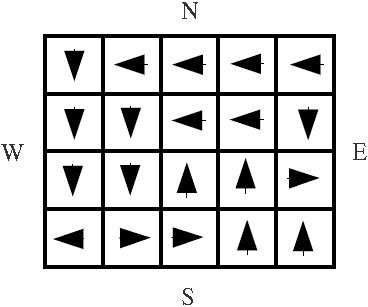
\includegraphics[width=0.45\textwidth]{../latex/img/1067/1067-1.png}
\end{figure}


เมื่อนำลูกบอลไปวางที่ช่องใด ลูกบอลจะถูกผลักไปในช่องถัดไปตามทิศทางของเครื่องกำเนิดสนามพลัง เมื่อถึงช่องถัดไป ลูกบอลก็จะถูกผลักไปในทิศทางของช่องนั้นอีก ไปเรื่อย ๆ จนกระทั่งลูกบอลเคลื่อนที่ออกนอกสนามพลัง ยกตัวอย่างเช่น ถ้าเริ่มวางลูกบอลที่ช่องคอลัมน์ที่ $5$ แถวที่ $1$ ลูกบอลจะเคลื่อนที่จนกระทั่งทะลุออกไปด้านข้างในทิศตะวันตกดังรูปซ้ายด้านล่าง อย่างไรก็ตาม ถ้าเริ่มวางลูกบอลที่บางตำแหน่ง เช่น ในคอลัมน์ที่ $4$ แถวที่ $3$ ลูกบอลจะเคลื่อนที่ไม่มีวันจบ


\begin{figure}[h!]
\centering
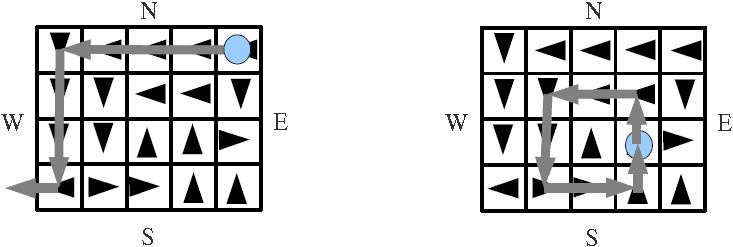
\includegraphics[width=0.7\textwidth]{../latex/img/1067/1067-2.png}
\end{figure}


\bigskip
\underline{\textbf{โจทย์}}  ให้เขียนโปรแกรมรับข้อมูลของสนามพลังและทิศทางของเครื่องกำเนิดสนามพลังแต่ละเครื่อง จากนั้นรับตำแหน่งเริ่มต้นของของลูกบอลแล้วคำนวณว่าลูกบอลจะวิ่งทะลุออกจากสนามในทิศทางใด หรือลูกบอลจะเคลื่อนที่ไม่รู้จบ

\InputFile

\textbf{บรรทัดแรก} ระบุจำนวนเต็มสามจำนวน คือ $N$ $M$ และ $K$ $(1 \leq N \leq 100; 1 \leq M \leq 100; 1\leq K\leq 20)$ โดยที่ $N$ และ $M$ แทนความกว้างและความยาวของสนาม $K$ แทนจำนวนลูกบอลที่ต้องคำนวณ

\textbf{บรรทัดที่ $2$ ถึง $M+1$} จะระบุข้อมูลของสนามพลัง กล่าวคือในบรรทัดที่ $r+1$ สำหรับ $1 \leq r \leq M$ จะมีจำนวนเต็ม $N$ จำนวน $a_1, a_2, ..., a_N$ แทนทิศทางของเครื่องกำเนิดพลังในแถวที่ $r$ โดยที่ $a_i$ จะระบุทิศทางของเครื่องกำเนิดพลังในคอลัมน์ที่ $i$ ทิศทางของเครื่องกำเนิดพลังจะแสดงในตารางด้านล่าง

\begin{center}
\begin{tabular}{|c|c|}
\hline
ค่าของ $a_i$ & ทิศ\\
\hline
1 & เหนือ (N)\\
\hline
2 & ตะวันออก (E)\\
\hline
3 & ใต้ (S)\\
\hline
4 & ตะวันตก (W)\\
\hline
\end{tabular}
\end{center}

\textbf{บรรทัดที่ $M+2$ ถึง $M+K+1$ }จะระบุตำแหน่งเริ่มต้นของลูกบอลลูกต่าง ๆ กล่าวคือ ในบรรทัดที่ $M + j +1$ สำหรับ $1 \leq j \leq K $ จะมีจำนวนเต็มสองจำนวน $X_j$ และ $Y_j$ $(1 \leq X_j \leq N; 1 \leq Y_j \leq M)$ แทนคอลัมน์และแถวเริ่มต้นของลูกบอลลูกที่ $j$

\OutputFile

\textbf{มี $K$ บรรทัด} ในบรรทัดที่ $j$ สำหรับ $1 \leq j \leq K$ จะมีผลลัพธ์ของลูกบอลลูกที่ $j$ โดยอาจมีค่าเป็นทิศทางที่ลูกบอลวิ่งออกจากสนามพลัง เป็นตัวอักษร N, E, S, และ W หรือเป็นข้อความ NO ถ้าลูกบอลวิ่งอยู่ในสนามพลังไม่รู้จบ


\Examples

\begin{example}
\exmp{2 2 2
2 2
2 1
1 1
1 2}{E
E}%
\exmp{5 4 2
3 4 4 4 4
3 3 4 4 3
3 3 1 1 2
4 2 2 1 1
5 1
4 3}{W
NO}%
\end{example}


\Source

การแข่งขัน YTOPC กุมภาพันธ์ 2552


\end{problem}

\end{document}